% This is samplepaper.tex, a sample chapter demonstrating the
% LLNCS macro package for Springer Computer Science proceedings;
% Version 2.20 of 2017/10/04
%
\documentclass[conference]{IEEEtran}
%
\usepackage{cite}
\usepackage{pslatex} % -- times instead of computer modern, especially for the plain article class
\usepackage[colorlinks=false,bookmarks=false]{hyperref}
\usepackage{booktabs}
\usepackage{graphicx}
\usepackage{xcolor}
\usepackage{multirow}
\usepackage{comment}
\usepackage{listings}

\usepackage{xspace}		% For using \SV with trailing spaces
\usepackage{cleveref}	% Needed for correctly referencing listings

\newcommand{\code}[1]{{\small{\texttt{#1}}}}
\newcommand{\SV}{SystemVerilog\xspace}


% fatter TT font
\renewcommand*\ttdefault{txtt}
\newcommand{\todo}[1]{{\color{olive} TODO: #1}}
\newcommand{\martin}[1]{{\color{blue} Martin: #1}}
\newcommand{\simon}[1]{{\color{green} Simon: #1}}
\newcommand{\andrew}[1]{{\color{red} Andrew: #1}}
\newcommand{\rewrite}[1]{{\color{red} rewrite: #1}}
\newcommand{\ducky}[1]{{\color{orange} Richard: #1}}
\newcommand{\kasper}[1]{{\color{purple} Kasper: #1}}
\newcommand{\hjd}[1]{{\color{pink} Hans: #1}}

% uncomment following for final submission
%\renewcommand{\todo}[1]{}
%\renewcommand{\martin}[1]{}
%\renewcommand{\simon}[1]{}
%\renewcommand{\kasper}[1]{}
%\renewcommand{\ducky}[1]{}


%%% ZF
\usepackage{listings}
\lstset{
	columns=fullflexible,
	%        basicstyle=\ttfamily\footnotesize,
	basicstyle=\ttfamily\small,      
	%columns=fullflexible, keepspaces=true,
	numbers=left,    
	numberblanklines=false,
	captionpos=b,
	%	breaklines=true,
	escapeinside={@}{@},
	numbersep=5pt,
	language=C,
	tabsize=2,
	breakatwhitespace=true,
	breaklines=true,
	deletekeywords={for},
	%        keywordstyle=\ttfamily
	numbersep=5pt,
	xleftmargin=.10in,
	%xrightmargin=.25in
}

\newcommand{\longlist}[3]{{\lstinputlisting[float, caption={#2}, label={#3}, frame=tb, captionpos=b]{#1}}}
\usepackage{graphicx}

% Used for displaying a sample figure. If possible, figure files should
% be included in EPS format.
%
% If you use the hyperref package, please uncomment the following line
% to display URLs in blue roman font according to Springer's eBook style:
% \renewcommand\UrlFont{\color{blue}\rmfamily}

\begin{document}
%
\title{Enabling Coverage-Based Verification in Chisel}
%\author{
%\IEEEauthorblockN{No Author Given}
%\IEEEauthorblockA{No Institute Given}
%}
%
%\titlerunning{Abbreviated paper title}
% If the paper title is too long for the running head, you can set
% an abbreviated paper title here

%\author{\IEEEauthorblockN{Andrew Dobis, Hans Jakob Damsgaard, Enrico Tolotto, Kasper Hesse, Tjark Petersen, Martin Schoeberl}}
\author{\IEEEauthorblockN{Andrew Dobis, Hans Jakob Damsgaard, Enrico Tolotto, \\
Kasper Hesse, Tjark Petersen, Martin Schoeberl}
\IEEEauthorblockA\textit{Department of Applied Mathematics and Computer Science} \\
\textit{Technical University of Denmark}\\
Lyngby, Denmark \\\\
\href{mailto:adobis@ethz.ch}{adobis@ethz.ch}, \href{mailto:hans.damsgaard@tuni.fi}{hans.damsgaard@tuni.fi}, \{\href{mailto:s190057@student.dtu.dk}{s190057}, \href{mailto:s183735@student.dtu.dk}{s183735}, \href{mailto:s186083@student.dtu.dk}{s186083}\}@student.dtu.dk, \href{mailto:masca@dtu.dk}{masca@dtu.dk}
%adobis@ethz.ch, hans.damsgaard@tuni.fi, s190057@student.dtu.dk, \\
%s183735@student.dtu.dk, s186083@student.dtu.dk, masca@dtu.dk
}

%\authorrunning{A. Dobis et al.}

% First names are abbreviated in the running head.
% If there are more than two authors, 'et al.' is used.
%
%\institute{Technical University of Denmark\\
%Department of Applied Mathematics and Computer Science\\
%Lyngby, Denmark\\
%\email{andrew.dobis@alumni.epfl.ch}, \email{s190057@student.dtu.dk}, %\email{s163915@student.dtu.dk}, \email{s183735@student.dtu.dk},\\
%\email{s186083@student.dtu.dk}, \email{masca@dtu.dk}\\}
%
\maketitle              % typeset the header of the contribution
%
%\martin{Title: Do we really restrict ourself to Chisel Designs? Maybe more general Digital Designs.}

\begin{abstract}
Ever-increasing performance demands are pushing hardware designers towards designing domain-specific accelerators. This has created a demand for improving the overall efficiency of the hardware design and verification cycles. The design efficiency was improved with the introduction of Chisel. However, verification efficiency has yet to be tackled.
One method that can increase verification efficiency is the use of various types of coverage measures.\\
In this paper, we present our open-source, coverage-related verification tools targeting digital designs described in Chisel. %We create a new method allowing for statement coverage at an intermediate representation of Chisel designs.
Specifically, we have created a new method allowing for statement coverage at an intermediate representation of Chisel, %We also describe our solution for gathering functional coverage on a Chisel design.
and several methods for gathering functional coverage utilizing the functional nature of Scala. We evaluate our approach by comparing it to existing coverage solutions from SystemVerilog.

\begin{IEEEkeywords}
Hardware Verification, Statement Coverage, Functional Coverage, Chisel, Scala.
\end{IEEEkeywords}

\end{abstract}

%\begin{itemize}
%    \item REVIEW 1 \todo{DONE} Add picture of language interactions.
%    \item REVIEW 2 \todo{TODO} Clarify contributions made by us. Otherwise, all good.
%    \item REVIEW 3 \todo{TODO} Clarify how to declare a verification plan. Provide more verification-related use case details and results. Be less harsh on "traditional" HDLs.
%    \item REVIEW 4 \todo{IRRELEVANT (or target another journal?)}
%\end{itemize}

%----------------------- REVIEW 1 ---------------------\\
%SCORE: 2 (accept)\\
%Moving the verification from the Verilog/Systemverilog to the Chisel stage, allows for a verification at an earlier stage and therefore makes it easier for the systemdesigner.
%Also the proposed algorithm allows the verifcation at various stages and therefore allows the systemdesigner to choice the best stage for a specific verification task.
%The paper is written in a nice and understandable way. The topic does not allow for many pictures and the authors tried their best, but a picture about the interactions between Verilog, FIRRTL, Chisel and its compilers would be nice.
%\martin{Already added by Andrew :-)}
%The addition of the proposed work to the chisel repository shows the value of this work.
%\martin{Nice, positive review}

%----------------------- REVIEW 2 ---------------------\\
%SCORE: 1 (weak accept)\\
%The paper describes an approach to add code coverage analysis to Chisel. Chisel is a high level hardware description language embedded in Scala. Unfortunatly, Chisel itself does not offer much functionality for code coverage. The authors first describe how code coverage can be done on the lower levels, since Chisel translates to FIRRTL and then to VERILOG. So code coverage analysis can be done on these two levels. Basic coverage is also provided on Chisel level, so the authors propose an extension to allow functional coverage analysis directly on Chisel level. This is an important approach. However, reading the paper I initially had difficulties to find out the contribution of the authors. More than 3/4 of the paper describe existing approaches before coming to the authors contribution. This is something that needs improvement, either by cutting out well known parts or at least by marking more clearly the authors' contribution. Nevertheless, since the topic is very interesting!
%g I weakly recommend the paper for acception.

%----------------------- REVIEW 3 ---------------------\\
%SCORE: -2 (reject)\\
%The paper describes approaches to improve the verification efficiency of hardware designs which use Chisel, FIRRTL or Scala specifications for design entry. Goal is to create coverage reports on statements and functions traversed in Chisel-based code during test runs. 
%
%The motivation of the authors, to help overcoming an inherent deficiency of Chisel-based design entries in terms of design verification, seems to be well founded. From this perspective, the submission could be of interest to the hardware design community. However, in terms of its scientific merits, the paper has a number of serious flaws:
%- Per the description in section 6, the verification plan with the specification of the cover points and bins has to be created manually. Methodology wise, how does this go beyond the straightforward specifications of manual test cases? How can this approach ensure that all necessary, pertinent cover points and bins are listed? The value of the outcome, the coverage report, entirely depends on the skill of the developer to specify the relevant cover points and bins. This is the known and old dilemma if designers write their own test specs. The doubts of the reviewer on the methodological novelty is also raised by the following sentence in the paper (last sentence before section 6.1): ``The concepts are directly taken from SystemVerilog, so it should be accessible to anyone coming from that environment.'' What's new here and goes beyond SystemVerilog?
%- The evaluation of the industry provided use case, a heap-based priority queue supporting scheduling tasks in real-time systems, falls very short. It is said that there are 5 cover points, each having up to 3 bins and 2 cross points each having up to 5 cross bins, being specified, but why is it necessary to specify exactly those points and bins in order to ensure coverage for the design at hand? I couldn't find any information that can be generalized for other designs, nor did I see any quantitative results reported for this use case.
%
%The value of the paper would be significantly improved if it could clarify what aspects of the verification plan generation process may be automated and supported by a corresponding tool, or how a tool could support the developer in formulating a comprehensive but not exhaustive verification plan. For the time being, the message is that the value of the coverage report entirely depends on the manually created verification plan. There is very little / no novelty in this ``method''. 
%
%The introduction declares the two most widely used HDLs as outdated and inefficient (kind of ignoring that SystemVerilog is the natural successor to Verilog - DRAM is also outdated, as all computing systems use DDR SDRAM these days, but its nevertheless DRAM). Authors might possibly rethink this general positioning of Chisel vs. other HDLS, as in the end, they are  "borrowing" verification concepts from exactly these HDLs - which is fully legitimate. For now, designers using SystemC or SystemVerilog for design entry rather see themselves confirmed in their choice.

%----------------------- REVIEW 4 ---------------------\\
%SCORE: -2 (reject)\\
%This paper extends the Chisel system to allow for verification. However, the paper is more into development or implementation rather than research, and thus find it hard to accept.
%\martin{We simply ignore this ignorant ``review''.}

\section{Introduction}
\label{sec:objectives}
As time passes, contemporary hardware design is met with tighter and tighter development and verification time-constraints. Additionally, hardware designers are turning to domain-specific accelerators in order to keep up with the ever-increasing performance demands~\cite{henn-patt:turing:2019}. This means that more and more hardware must be designed from scratch in shorter and shorter time periods~\cite{domain-hw-acc:2020}.  To help meet these demands, researchers at the University of California in Berkeley proposed Chisel~\cite{chisel:dac2012}, a Scala embedded high-level hardware construction language.

This solution is powerful, but is still lacking in verification functionalities. One of the main tools needed for the verification of digital systems is coverage. This allows verification engineers to measure their progress throughout the testing process and have an idea of how effective their tests actually are. Coverage can be separated into multiple distinct categories, but we will focus on the following two: statement and functional coverage. Statement coverage defines a measure for \textit{``how many code statements have been tested?"}, whereas functional coverage gives a measure for \textit{``which functionalities have been tested?"}~\cite{spear2008systemverilog}.

%\martin{shall write some words on the different languages levels.}

In this paper, we explore how to use existing tools, both for Scala and for Verilog, in order to obtain statement coverage in Chisel. We will start by presenting code coverage at the Scala level. Second, we will briefly discuss how to use Verilator~\cite{verilator} in order to enable statement coverage of the generated Verilog description. Third, we will show our solution for getting statement coverage of the so-called Flexible Internal Representation of Register Transfer Level (FIRRTL) intermediate representation~\cite{firrtl}. In total, these measures represent test coverage of different language levels of a Chisel design.

Moreover, we will present our solution for gathering functional coverage of a Chisel design directly in Scala. %We provide a brief introduction to Chisel and FIRRTL needed to fully appreciate our solution. Initial work on verification with Chisel has been presented in a previous paper~\cite{blind}. %\cite{verify:chisel:2020}. 
Finally, we evaluate our coverage solutions with an industry-provided use case to illustrate its efficiency. The solutions are shown to reduce the amount of code (measured in lines of code) needed to gather functional coverage on a Chisel design in comparison to using SystemVerilog extended by Universal Verification Methodology (UVM) techniques~\cite{uvm2015}.
%Note that a discussion could be had on the usefulness of coverage information at certain levels of abstraction (i.e. high-level coverage might not be interesting when using hardware generators), but for now this is left up for the reader to decide.

The contributions of this paper are a method for extending FIRRTL execution engines for gathering statement coverage, 
as well as novel tools and methods for defining and gathering functional coverage in a high-level hardware construction language such as Chisel.

The paper is organized as follows.
The following section presents related work.
Section III presents background on Chisel and various coverage methodologies. 
Section IV discusses how existing tools can be used to gather statement coverage of a Chisel design.  
Section V presents our work on adding statement coverage at the FIRRTL level. 
Section VI then presents our Scala-based functional coverage framework.  
In section VII, we evaluate our solution by comparing to similar tests written in SystemVerilog with UVM. 
Section VIII concludes.

\section{Related Work}

%\martin%\martin{The references are too many web links and too few papers.}

SystemVerilog, a mostly non-synthesizable extension of the Verilog Hardware Description Language (HDL), contains certain constructs capable of gathering coverage information~\cite{spear2008systemverilog}. These can be used when working with the Verilog description generated by Chisel. Developers of the Chisel language have added \texttt{cover} statement in an experimental verification library as part of the Chisel 3.4.0 release~\cite{chisel3.4release_notes}. This \texttt{cover} statement was then given an equivalent at the FIRRTL level, which then maps down to SystemVerilog rather than plain Verilog. There is yet to be mainstream support for this new construct by FIRRTL execution engines like Treadle\footnote{Available at \url{https://github.com/chipsalliance/treadle}}, which would explain why it remains experimental. Our solution greatly differs from this approach, since we utilise pre-existing language features from Chisel/Scala in order to enable coverage in the simplest possible manner. Additionally, our functional coverage solution allows for greater customizability in terms of the behavior captured by the different cover constructs, while Chisel's \texttt{cover} statement is limited by a simple predicate evaluated on sampling.   
  
A possible solution to obtaining statement coverage for Chisel, is to rely on the generated Verilog code. 
%This can be simulated by any Verilog simulator or directly synthesized by any vendor-specific development tool. 
As part of the Chisel development tools, \texttt{ChiselTest} allows simulating a Chisel design transformed to Verilog using the open-source Verilator~\cite{verilator} back-end.
Some coverage metrics can be enabled using a few simulation parameters in Verilator~\cite{tolotto2020}.
The simulator then generates a coverage report in a SystemPerl coverage report file~\cite{SystemPerl}.

SystemVerilog is widely used in the scope of UVM~\cite{uvm2015}. 
Using SystemVerilog, a verification plan may be defined using the following constructs: \texttt{Bin}, which defines a range of values that should be tested for, \texttt{CoverPoint}, which defines a port that needs to be sampled in the coverage report and \texttt{CoverGroup}, which defines a set of \texttt{CoverPoint}s that need to be sampled at the same time. 
SystemVerilog also supports cross coverage, a special kind of \texttt{CoverPoint} where a hit is only considered when two or more \texttt{CoverPoint}s have specific values at the same time.
Coverage is sampled whenever the \texttt{sample} method is called on a \texttt{CoverGroup}. 
%Once the test has been run, a coverage report may be generated by the simulator. 
In contrast to this, our solution offers tools which allow for a more customizable verification plan, enabling a definition that closely models the target specification.

In relation to timed coverage, Property Specification Language (PSL) and the similar SystemVerilog Assertions (SVA)~\cite{Boule2008} are two current solutions allowing for the use of temporal logic in relation to both coverage and assertions. 
PSL for example offers a wide variety of Sequential-Extended Regular Expressions (SEREs), which define temporal relations between different boolean expressions, ranging from SERE concatenation \texttt{;}, matching two expressions at consecutive cycles, to \texttt{within}, matching one expression as a temporal subset of another, and many more. This language also has extensions adding other functionalities from Linear-Temporal Logic (LTL), such as the \texttt{past}~\cite{Dax2010:temporal-logics}. These solutions are both quite complex and require the use of many operators to describe what could be a simple temporal relation. Rather than relying solely on temporal operators to express a form of LTL, our solution aims to provide a simplified set of temporal constructs that encompass a similar range of temporal relations when used in conjunction with our different types of bins.

We defend the idea of creating verification methods in Scala (in open-source), rather than relying on an external language, since it improves the overall cohesion of the Chisel/Scala ecosystem. 
This thus saves the verification engineers time and improves overall efficiency of the verification process, which is our main goal. 
Following that same idea, we briefly mention the work conducted in parallel to the research presented in this paper on constructing a hardware verification library for Chisel entirely in Scala, namely \texttt{ChiselVerify}~\cite{ChiselVerify:dobis2021}.

\section{Background}
\label{sec:background}
We begin by presenting a brief overview of Chisel and FIRRTL. 
After that, we will give an introduction to statement and functional coverage.

%\martin{This is probably too long. And State-of-the-Art should be in related work.}

\subsection{Chisel}
Chisel is a hardware construction language embedded in the functional and object-oriented programming language Scala~\cite{chisel:dac2012, chisel:book, Scala}. 
A Chisel design generates a Verilog description that can then be synthesized using existing tooling. 
Chisel syntax is rooted in Scala. As a result, it enables the description of hardware in a high-level manner. 
Scala also allows for both functional and object-oriented programming constructs, which makes it possible to organize a design very intuitively using Scala classes and objects, and to use the power of higher-order functions to simplify descriptions thanks to constructs like \textit{mappings} or \textit{reductions}.

\begin{figure*}[t]
    \centering
    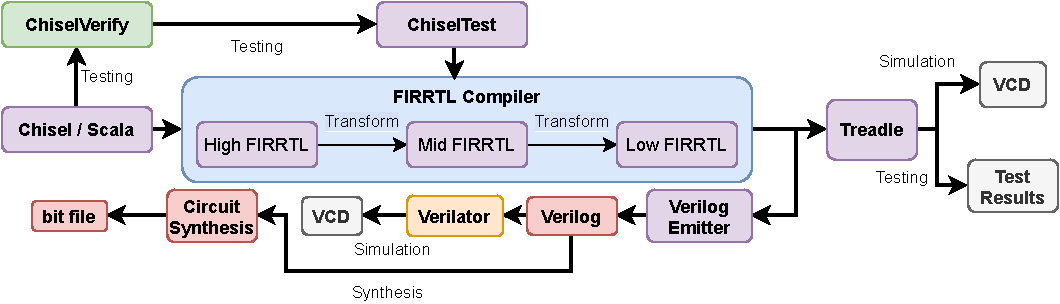
\includegraphics[width=0.8\textwidth]{Chisel_FIRRTL_VERILOG.pdf}
    \caption{Overview of the Chisel pipeline. Chisel code is first given to the FIRRTL compiler, where it is transformed by a series of ``lowering passes''. It is then output by the compiler in a low-level form, where only hardware primitives are used without loops. It is then used to either emit Verilog or simulate using an execution engine like Treadle.}
\label{fig:chisel}
\end{figure*}

\subsection{FIRRTL}
In a Chisel design, the source code is first compiled into an intermediate representation named FIRRTL. 
This is used as a sort of ``optimization layer" before being converted into the final Verilog form. 
During this optimization process the original Chisel description goes through three different intermediate representation layers:
\begin{itemize}
\item High-FIRRTL, which is a form that maps perfectly back to Chisel, but with the FIRRTL structure.
\item Mid-FIRRTL, which is a form where abstract constructs are simplified, i.e., loops are unrolled and arrays are flattened.
\item Low-FIRRTL, which maps to RTL code with high-level conditional statements turned into multiplexers.
\end{itemize}
Throughout this optimization process, custom FIRRTL compiler passes, known as \textit{Transforms}, can be used to modify the design. 
This is often done when trying to apply simplifications to the design to make the generated hardware more optimal~\cite{firrtl}.  

Figure~\ref{fig:chisel} shows an overview of the Chisel compilation pipeline and the different stages the code goes through before being converted into a usable format. It also indicates the placement of our coverage tools as part of the \texttt{ChiselVerify} package.

\subsection{Test Coverage}
In software development, test coverage is used as a metric to measure the completeness of a testing suite. 
In recent years, these techniques, originally used for software, have been brought into the hardware verification universe. 
In this paper, we will mostly focus on two key approaches to test coverage: statement coverage and functional coverage. 
%Nonetheless, we briefly mention closely related and more thorough coverage metrics here.

\paragraph{Statement Coverage} When wanting to retrieve coverage information about a specific design, statement coverage will give a quantitative measure of our testing progress. It measures which percentage of statements in our code have been executed during the test. This metric is widely used in the software world and may be ported directly to the hardware world. However, it should be taken with a grain of salt and not as the sole metric for how thorough one's testing was, since it only provides information about which lines were tested and not how well they were tested~\cite{hdlverify}. %This metric can be very useful in the software world, however it is only a partial solution in the hardware world, since it only tells us which lines were tested and not how well they were tested. 

%Related metrics are line and block coverage. Line coverage measures execution of specific code lines. For languages that are less expressive than Scala (such as C), line and statement coverage are equivalent. Block coverage simply reduces the granularity focusing on sections of code at once. Depending on the language, blocks may be explicit or implicit~\cite{hdlverify}. %For example, consider the code snippets below. The left Verilog snippet presents an explicit block surrounded by an \texttt{if}-statement whose check may never be true, while the right VHDL snippet presents an implicit block starting with the \texttt{wait}-statement which may never be passed~\cite{hdlverify}.

%\noindent\begin{minipage}{0.45\linewidth}
%\begin{lstlisting}[language=verilog]{verilogBlock}
%if (dtack == 1'b1) begin: acked
%    as <= 1'b0;
%    data <= 16'hZZZZ;
%    bus_rq <= 1'b0;
%    state <= IDLE;
%end
%\end{lstlisting}
%\end{minipage}\hfill
%\begin{minipage}{0.45\linewidth}
%\begin{lstlisting}[language=vhdl, firstnumber=1]{vhdlBlock}
%address <= h"FFED";
%ale     <= '1';
%rw      <= '1';
%wait until dtack = '1';
%read_data := data;
%ale     <= '0';
%\end{lstlisting}
%\end{minipage}

%More elaborate metrics include path and expression coverage. Figure~\ref{fig:expr} shows examples of both. Path coverage focuses on whether all possible paths through a piece of code have been executed. 
%Expression coverage takes this one step further checking whether all possible combinations of true checks are executed. The left code snippet in Figure~\ref{fig:expr} shows an example of path coverage, while the right code snippet shows expression coverage. One must note that the finer the granularity, the greater the computational requirements~\cite{hdlverify}. %For simple designs, statement coverage is generally sufficient. \hjd{Check up on this and explain more.}
%
%\begin{figure}
%    \centering
%    \includegraphics[width=0.5\textwidth]{Coverage_example.pdf}
%    \caption{Example of (left) path and (right) expression coverage.}
%\label{fig:expr}
%\end{figure}

\paragraph{Functional Coverage} If we are looking to measure the completeness of a test suite, we need to ask the following question: \textit{``are we even testing the right thing?"}. 
In the hardware world, engineers usually implement designs based on pre-determined specifications, so when testing, we should also have a metric for how well we are implementing the specification. 
Functional coverage is that metric. 
The idea is to first define what is called a \textit{verification plan}~\cite{spear2008systemverilog}, which represents the specification we are implementing. 
A good verification plan tests only the required functionality of a DUT. As such, it should apply only 
realistic input patterns to the DUT.
Once a plan is defined, we sample the different points defined in the specification during the testing process to obtain results in the form of: \textit{``test suite T covered a total of x\% of the values specified by point P in specification A"}. 

\subsection{What to Aim For}
The greatest pitfall is the idea of needing to achieve 100\,\% statement coverage. Indeed, for the majority of cases, reaching 100\,\% statement coverage is unreasonable due to computational requirements or impossible due to statements not meant to be executed. Instead, one should aim for fully exercising the most important features of one's design; thus, targeting high functional coverage. Statement coverage can still be useful, however, as it indicates whether sections of one's code are not executed. 

Additionally, one should keep in mind that coverage metrics only indicate the thoroughness of one's verification suite, neither its correctness nor its completeness. Designing a good verification plan is therefore of the utmost importance~\cite{hdlverify}.

\subsection{Coverage in Chisel} 
%Up until recently, the main Chisel developers have mostly focused their energy on getting Chisel up to the standards imposed by mainstream HDLs like VHDL or Verilog. 
Verification features are mostly lacking from the Chisel package. 
The most common way to test a design implemented in Chisel, is by using \texttt{ChiselTest}~\cite{chisel:tester2}. 
This is a testing framework for Chisel that gives access to a simple \texttt{peek}, \texttt{poke} and \texttt{expect} testing interface. 
\texttt{ChiselTest} also helps the user create golden models, to test their design against, entirely in Scala or by using the Java Native Interface (JNI) with already defined models written in, e.g., C. This is further supported by a simple \texttt{fork} functionality for easy concurrency.  
This framework, however, is lacking in verification functionalities and does not give the user any way to gather coverage on a Chisel design.
Hence, if one wants to gather test coverage on a current Chisel design, they need to rely on basic Scala software coverage tools (which we explore in more detail in the next section). 
We are, therefore, introducing coverage solutions that are specifically tailored for Chisel.

\section{Applying an Existing Tool}
We will start with measuring coverage at a high level (i.e., coverage of the Scala/Chisel code itself). Scala and its corresponding software testing framework ScalaTest have some coverage functionalities built-in, specifically, we have looked at the Scoverage plugin~\cite{scoverage}. Scoverage supports statement and branch coverage. We note that according to the Chisel3 GitHub page, Scoverage should work with Chisel~\cite{chisel:scoverage}.

%%\martin{This actually does coverage of the Chisel hardware generation, not the Chisel hardware itself. It tests the generator, which is important as well.} Fixed.

To enable coverage, the Scoverage plugin must be added to the Scala project, including optional arguments.
%'s \textit{plugins.sbt} file, and a number of optional arguments may be included in the project's \textit{build.sbt} file -- the arguments specify whether coverage is enabled, a targeted coverage percentage, etc.
%An example configuration of the Scoverage plugin is provided below:
%\begin{verbatim}
%coverageEnabled := true
%coverageMinimum := 70
%coverageFailOnMinimum := false
%coverageHighlighting := true
%\end{verbatim}
% Running a test is still just a matter of running e.g. \texttt{sbt test}, while generating a coverage report requires running \texttt{sbt coverageReport} afterwards, as Scoverage otherwise simply generates coverage databases.
Running the test and coverage reporter tool will create a graphical coverage report in a set of HTML files. The report may optionally include the original source files with statements that were executed during the test marked in green. The global coverage results are also printed to \texttt{stdout}.
%in the terminal:
%\begin{verbatim}
%[info] Statement coverage.: 100.00%
%[info] Branch coverage....: 100.00%
%\end{verbatim}

While this sounds promising, experimenting with Scoverage in combination with Chisel revealed some limitations. In particular, some of the basic constructs introduced by Chisel, e.g. \texttt{switch} statements, are simply not considered by the coverage tool and thus, incomplete results are reported. In practice, this makes Scoverage insufficient for hardware verification. However, it must be noted that Scoverage provides coverage results for the hardware generators written in Chisel, which can also be important to consider, both for verification and potentially for optimization purposes by pointing a designer's attention toward unused generator code.

\section{Statement Coverage at the FIRRTL Level}  
%Let us now move down an abstraction level and discuss how we've gone about implementing statement coverage at the FIRRTL level. First of all, we must briefly discuss the utility of having coverage at an intermediate representation level.
Statement coverage at the FIRRTL level is interesting for two reasons; first, FIRRTL is intuitively mapped back to the Chisel code, and second, it contains only expanded hardware code meaning that we obtain coverage information on the generated hardware rather than the hardware generators.%FIRRTL is a direct translation of the input Chisel source, meaning that it can be mapped intuitively back to the designer's code. An argument for the usefulness of coverage information at such an abstraction level is the fact that in FIRRTL, all hardware generators are expanded, meaning that we obtain coverage information on the generated hardware rather than the hardware generating code. 

Thus, to enable this, we developed a new method allowing for coverage measurements in Treadle, a common FIRRTL execution engine used to simulate Chisel designs with the \texttt{ChiselTest} framework. We do so by running tests through an extended version of Treadle (available as a SNAPSHOT at the time of writing).%We developed a new method allowing for coverage measurements in Treadle, a common FIRRTL execution engine used to simulate designs implemented in Chisel. This engine runs on the FIRRTL intermediate representation code generated by a given Chisel implementation and allows to run user-defined tests on the design, using frameworks like \texttt{iotesters} or the more recent \texttt{ChiselTest}. One way to obtain FIRRTL-level statement coverage would be to run our tests through an extended version of Treadle (available through a SNAPSHOT at the time of writing) capable of keeping track of the necessary information.

Baxter describes a method for collecting statement coverage for arbitrary languages~\cite{branch-cov-made-easy:2002}, which we adapt for Hardware Description Languages. 
The idea is to extend each multiplexer of a design with additional outputs. 
These new ports, known as coverage validators, are set depending on the paths taken by each multiplexer. 
During testing, the ports are sampled and used for checking whether a certain multiplexer path was taken. 
This results in a particular branch coverage percentage which can be mapped to a statement coverage percentage.

%\martin{Baxter should be in related work. Not stating here that we base on it.}
Baxter describes a method for collecting statement coverage for arbitrary languages~\cite{branch-cov-made-easy:2002}, which we adapt for Hardware Description Languages. 
The idea is to extend each multiplexer of a design with additional outputs, known as coverage validators, which are set depending on the paths taken by each multiplexer
During testing, the ports are sampled and used for checking whether a certain multiplexer path was taken. 
This results in a particular branch coverage percentage which can be mapped to a statement coverage percentage.

We implement this by simply extending each multiplexer in the expanded FIRRTL code by the required extra ports. %. The idea is to extend each multiplexer in the design by additional outputs. These new ports, known as coverage validators, are set depending on the paths taken by each multiplexer. These ports are then sampled during testing and used for checking whether a certain multiplexer path was taken. This results in a particular branch coverage percentage which may be mapped to a statement coverage percentage.%The solution that was used to implement statement coverage is based on a method presented by Baxter~\cite{branch-cov-made-easy:2002}. The idea is to add additional outputs for each multiplexer in the design. These new ports, which we will call \textit{Coverage Validators}, are set depending on the paths taken by each multiplexer. That information is then gathered at the end of each test and maintained throughout a test suite. Once the testing process is finished, we use the output values gathered from the \textit{Coverage Validators} to check whether or not a certain multiplexer path was taken during the test, resulting in a branch coverage percentage. This percentage can then be mapped to a statement coverage percentage.
As such, our implementation is based on a custom pass of the FIRRTL compiler that traverses the source's abstract syntax tree and adds the additional outputs and coverage expressions as needed. During a test, the outputs are sampled on each call to the \texttt{expect} method. Finally, the results are compiled to a Scala \texttt{case class} containing:%We developed this method inside of Treadle by creating a custom pass of the FIRRTL compiler, in Scala, that traverses the source's abstract syntax tree and adds the additional outputs and coverage expressions into the data structure. Once that is done, the \texttt{TreadleTester} samples those additional outputs every time the \texttt{expect} method is called and keeps track of their values throughout a test suite. Finally, it generates a Scala \texttt{case class} containing the following coverage information:
\begin{itemize}
\item The multiplexer path coverage percentage.
\item The Coverage Validator lines that were covered by a test.
\item The modified LoFIRRTL source code in the form of a \texttt{List[String]}.
\end{itemize}
The case class may be serialized into a coverage report. The report contains annotated LoFIRRTL code lines marked by ``\texttt{+}'' if they have been executed at least once during the tests and ``\texttt{-}'' otherwise. A component's input/output ports are, per default, considered executed. Hence, ``\texttt{-}'' can only appear on lines containing a coverage validator as it represents a non-explored multiplexer path. Consider for example the following report of a simple circuit in which only the path for which \texttt{io\_a} is 1 has been tested:
%The \texttt{CoverageReport} case class can then be serialized, giving the following example report:
\begin{verbatim}
COVERAGE: 50.0% of multiplexer paths tested
COVERAGE REPORT:

+ circuit Test_1 :
+   module Test_1 :
+     input io_a : UInt<1>
+     input io_b_0 : UInt<2>
+     input io_b_1 : UInt<2>
+     input clock : Clock
+     output io_cov_valid_0 : UInt<1>
+     output io_cov_valid_1 : UInt<1>
+     output out : UInt<2>
+   
+     io_cov_valid_0 <= io_a
-     io_cov_valid_1 <= not(io_a)
+     out <= mux(io_a, io_b_0, io_b_1)
\end{verbatim}
%The example above is taken from a simple test, where we are only testing the path where \texttt{in\_a} is 1. This means that, since we only have a single multiplexer, only half of our branches have been tested.
% The report can thus be interpreted as follows:  
%\begin{itemize}
%\item ``\texttt{+}" before a line, means that it was executed in at least one of the tests in the test suite. All port declarations are considered explored by default.
%\item ``\texttt{-}" before a line, means that it wasn't executed in any of the tests in the test suite. This can only appear next to a line containing a coverage-validator, since it represents a non-explored multiplexer path.
%\end{itemize}

%With our modification Treadle thus allows us to obtain Statement coverage at the FIRRTL level. 

%\martin{Maybe we should lookup what Kevin is doing. Kind of picked up our work.}

\section{Functional Coverage in Chisel}
As described previously, statement coverage is not sufficient for verifying complex hardware. As such, a tool for hardware verification would not be complete without constructs allowing one to define a verification plan and retrieve a functional coverage report from it. %Functional coverage is one of the principal tools used during the verification process. It allows one to measure \textit{``which part of the specification has been implemented correctly"}. A discussion on hardware verification would thus not be complete without constructs allowing one to define a verification plan and retrieve a functional coverage report. 

A verification plan informs a coverage reporter which ports should be sampled and kept track of in the coverage report. In SystemVerilog and UVM, verification plans are based on three elements: \texttt{Bin}s, \texttt{CoverPoint}s and \texttt{CoverGroup}s. We take a similar approach but extend upon their functionality. As such, we need to be able to do the following: %Functional coverage is based on three base elements: \texttt{Bins}, \texttt{CoverPoints} and \texttt{CoverGroups}. Using these, one can define what is known as a verification plan, which tells the coverage reporter which ports need to be sampled and taken into account in the coverage report.
%In order to implement said elements in Scala, we needed to be able to do the following:
\begin{itemize}
\item Define a verification plan. %(using constructs similar to \texttt{coverpoint} and \texttt{bins}).
\item Sample DUT ports.%(for example by hooking into the \textit{ChiselTest} framework).
\item Keep track of the number of hits in each bin.% (using a sort of a database).
\item Compile the results into a comprehensible report.%Compile all of the results into a comprehensible coverage report.
\end{itemize}

We implemented this on top of the existing \texttt{ChiselTest}~\cite{chisel:tester2} framework with a top-level \texttt{CoverageReporter} class whose \texttt{register} method is used to define verification plans. Internally, the coverage reporter stores \texttt{CoverPoint} to \texttt{Bin} mappings inside a \texttt{CoverageDB}. Once defined, the \texttt{sample} method (based on \texttt{ChiselTest}'s \texttt{peek} method) is used to update bins. After a test, a coverage report can be generated using the \texttt{printReport} method. Our solution extends existing tools with special coverage constructs that allow the user to define relations between ports. %We implemented this on top of the existing \texttt{ChiselTest}~\cite{chisel:tester2} framework. We start with a top-level construct, called \texttt{CoverageReporter}, which allows one to define a verification plan using the \texttt{register} method, which itself stores \texttt{coverpoint} to \texttt{bin} mappings inside of a \texttt{CoverageDB}. Once the verification plan is defined, we can sample the DUT ports using the \texttt{sample} method, which hooks into \texttt{ChiselTest} in order to use its peeking capabilities. At the end of the test suite, a functional coverage report can be generated using the \texttt{printReport} method, which shows us how many of the possible values, defined by our bin ranges, were obtained during the simulation.
%Our solution also enables the use of special \texttt{Cover} constructs that allow the user to define relations between ports.

\subsection{Cross Coverage}
Basic coverage relations between multiple ports can be defined using a \texttt{CrossPoint}. 
This allows one to associate a set of ports to a set of ranges of equal size.  
A sample of the ports is considered a hit if all of the port values are contained in their associated ranges. This is particularly useful for checking whether all interesting combinations of values on a set of ports were tested~\cite{hdlverify}. An example being injection of valid and corrupt packets on all ports of a NoC router. %A hit is then considered if each of the ports was sampled with a value that is contained in its associated range.  
%Using this construct, the user has a way to gather information about the interactions between multiple ports.  

\subsection{Timed Coverage}
Timed coverage relations in our solution aim to provide a simple and accessible form of temporal logic related to functional coverage. Adding a temporal argument to our \texttt{cover} construct allows to define relations between ports sampled at different cycles. The user specifies the expected delay and temporal construct to use. For this, we provide the following three basic operators, which we call delay types:%\texttt{TimedCross} constructs offer the possibility to gather delayed coverage relationships between two ports. The idea is similar to how a \texttt{CrossPoint} works, but rather than sampling both points in the same clock cycle, we look at the relation between one point at the starting clock cycle and another point sampled a given number of clock cycles later. This is defined by the \texttt{delay} and there are three different ways to specify it:  
\begin{itemize}
 \item \texttt{Exactly}, a hit will only be considered if the second point is sampled in its range at exactly the given number of cycles after the first point was.
 \item \texttt{Eventually}, a hit will be considered if the second point is sampled in its range at any point within the given number of cycles after the first point was.  
 \item \texttt{Always}, a hit will be considered if the second point is sampled in its range during every cycle for a given number of cycles after the first point was.
\end{itemize}  
The delay types are illustrated in figure~\ref{fig:delay}. Green dots indicate when the second point must be sampled in its range for it to be considered a hit. %Using these constructs, one can add timing-based information to the verification plan.

\begin{figure}
    \centering
    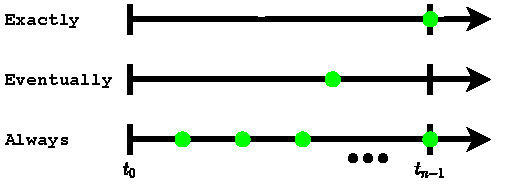
\includegraphics[width=.8\linewidth]{TimedCoverage.pdf}
    \caption{Illustration of the three delay types supported by our coverage tools.}
    \label{fig:delay}
\end{figure}

\subsection{Conditional Coverage} \label{sec:conditional_coverage}
Working in Scala allows us to use functions as higher-order objects. 
%This means that we can have bins that are defined using arbitrary predicates rather than specific value ranges. 
We exploit this and provide a \texttt{CoverCondition} construct which may be used to gather coverage information on an arbitrary number of ports with a user-defined predicate. %This was thus enabled with our \texttt{CoverCondition} object.
%This object gathers coverage information on an arbitrary number of ports by using user-defined predicates in order to consider Bin-hits.
 A sample is considered a hit if the predicate evaluates to \texttt{true}. %This means that a hit is considered when the predicate evaluates to \texttt{true}. 
 Since we are working with an arbitrary number of ports, computing the set of possible value combinations in order to obtain a coverage percentage is computationally expensive. 
To alleviate said problem, we added an optional \texttt{expectedHits} parameter that lets the user define a number of expected hits to generate a coverage percentage. If passed, the coverage report will include a hit percentage for the particular \texttt{CoverPoint}. Otherwise, no percentage is included.
%This is then used to compute the coverage percentage.
This coverage information can be very useful when wanting to create points that cover sparse ranges.   
We also provide this predication functionality for regular bins to enable them to have non-trivial ranges, e.g., covering only odd numbers in the range $[0,100)$ with condition \texttt{\{ case Seq(x) => x \% 2 != 0 \}}.%This sort of predication can also be used in conjunction to a regular bins to create a predicate that is only evaluated over a specific range.  

\subsection{Example Verification Plan and Coverage Report}%\subsection{Creating a Verification Plan}
%The basic verification plan semantics are as follows:
%\begin{itemize}
%    \item \texttt{CoverGroup} is defined as a set of \texttt{CoverPoint}s using the \texttt{cr.register} method.
%    \item \texttt{CoverPoint} is defined as a set of \texttt{Bins} tied to a DUT port and a name. If no \texttt{Bins} are given, then a \texttt{DefaultBin} is used, ranging over all possible values for the given port.
%    \item \texttt{Bins} is defined by a name and a value range.
%    \item \texttt{CrossPoint} is defined by an arbitrary number of ports and a list of \texttt{CrossBins}.
%    \item \texttt{CrossBin} is defined using the same number of ranges as the number of ports in the parent \texttt{CrossPoint}.
%    \item \texttt{TimedCross} is defined using two ports, a set of cross bins and a delay.
%    \item \texttt{CoverCondition} is defined using an arbitrary number of ports and a predicate.
%\end{itemize}
Using the aforementioned elements, users can define accurate representations of their specifications in the form of verification plans. The following listing shows an example verification plan utilizing all of the tools to verify a device under test (DUT) denoted \texttt{dut}: 
\begin{lstlisting}[language=scala]
val cr = new CoverageReporter(dut)
cr.register(
  cover("accu", dut.io.accu)(
    bin("lo10", 0 until 10),
    bin("First100odd", 0 until 100,
      { case Seq(x) => x % 2 != 0 }))),
  cover("aAndB", dut.io.outA, dut.io.outB)(
    bin("asuptobAtLeast100", 
      condition = { case Seq(a, b) => a > b }, 
      expectedHits = 100),),
  cover("accuAndTest", dut.io.accu, dut.io.test)(
    cross("both1", Seq(1 to 1, 1 to 1))),
  cover("timedAB", dut.io.outA, dut.io.count)(Exactly(3))(
    cross("ExactlyBoth3", Seq(3 to 3, 3 to 3))) 
)
\end{lstlisting}
%The above code snippet shows an example of how to define a verification plan using the presented framework.

%\subsection{Generating the Coverage Report}
During the subsequent tests, we must call \texttt{cr.sample()} whenever we wish to sample the defined \texttt{CoverPoint}s. %After defining a verification plan, we need to decide when we want to sample our cover points. This means that, at some point in our test, we have to tell our \texttt{CoverageReporter} to sample the values of all of the points defined in our verification plan. 
%This can be done simply by calling \texttt{cr.sample()} when we are ready to sample our points. 
Once our tests are done, we can ask for a coverage report by calling \texttt{cr.printReport()}, which results in the following: 
\begin{verbatim}
============== COVERAGE REPORT ==============
================ GROUP ID: 1 ================
COVER_POINT PORT NAME: accu
BIN lo10 COVERING Range 0 until 10 
HAS 8 HIT(S) = 80%
BIN First100odd COVERING Range 0 until 100 
WITH CONDITION onlyOdd HAS 1 HIT(S) = 1,00%
============================================
COVER_CONDITION NAME: aAndB
CONDITION asuptobAtLeast100 HAS 5 HITS 
EXPECTED 100 = 5.0%
============================================
CROSS_POINT accuAndTest FOR POINTS accu AND test
BIN both1 COVERING Range 1 to 1 CROSS Range 1 to 1 
HAS 1 HIT(S) = 100%
============================================
CROSS_POINT timedAB WITH AN EXACT DELAY OF 3
BIN ExactlyBoth3 COVERING: CROSS(Range 3 to 3, 
Range 3 to 3) HAS 1 HIT(S) = 100,00%
============================================
============================================
\end{verbatim}
The above report shows each point with its user-defined name and the bins it contains. These are then associated to a number of hits and, whenever possible (as described in section~\ref{sec:conditional_coverage}), a coverage percentage.
Another option would be, for example if we want to do automated constraint modifications depending on coverage results, to generate the coverage report as a Scala \texttt{case class} and then to use its \texttt{binNcases} method to get numerical and reusable coverage results.  

\section{Evaluation}
%\todo{Expand efficiency measure beyond LOC. Possibly in API complexity or similar.}
%%\martin{Could be more} \hjd{Let's switch to the Leros AluAccu that Kasper has written a UVM test for.}
To evaluate our new coverage tools that we include in our \texttt{ChiselVerify} package, we will verify an ALU accumulator module which is found at the center of processors implementing the Leros ISA~\cite{leros:comp:2019}. We first use our Scala coverage tools and then compare to the same done using SystemVerilog with UVM. %To evaluate our new Coverage tools, we will verify an accumulator ALU for the Leros ISA~\cite{leros:comp:2019} using at first our Scala coverage tools, then compare it to the same done using SystemVerilog with UVM.  
 The ALU accumulator supports operations such as \texttt{add}, \texttt{load}, \texttt{shiftRight} and bitwise operations. %The ALU is a simple accumulator, that supports operations such as \texttt{add}, \texttt{sub}, \texttt{and}, \texttt{or}, \texttt{xor}, \texttt{load} and \texttt{shiftRight}.   
 In order to test this entirely, we need to try all operations on the \texttt{op} input and all input value corner cases on the \texttt{din} input. %In order to test this entirely, we would need to try all operations, defined by the \texttt{op} input, and all corner cases for the input values, using the \texttt{din} input.  
 A good verification plan would thus capture what we just described.  
%cr.register(
%	cover("reset", dut.io.reset, dut.io.op) (Exactly(1)) (
%		cross("zeroToOne", 0 to 1, defaultRange(dut.io.op))))
\begin{lstlisting}[language=scala] 
val cr = new CoverageReporter(dut)  
cr.register(
  cover("ops", dut.io.op)(DefaultBin(dut.io.op)),
  cover("dataInputs", dut.io.din)(
    bin("minValue", Integer.MIN_VALUE),
    bin("neg1", -1),
    bin("zero", 0),
    bin("one", 1),
    bin("maxValue", Integer.MAX_VALUE)
  )
)
\end{lstlisting}
In the above code snippet, we registered a \texttt{CoverGroup} that ensures that the edge cases of all operations are tested.
Here, the implicit \texttt{defaultRange} and \texttt{DefaultBin} functions are used to cover all possible values for the \texttt{dut.io.op} port.
All that is left now is to call \texttt{cr.sample()} once per cycle in our \texttt{ChiselTest} test class.

%\martin{I am not sure if we should show UVM code here.}
In order to do the same with UVM, we need to:  
\begin{itemize}
    \item Create a UVM-subscriber based coverage class.
    \item Instantiate the current DUT. %(\texttt{LerosAlu lalu = new;})
    \item Declare the verification plan.
    %covergroup cg_post_rst;
%	UPDOWN: coverpoint cmd.reset {
%		bins updown = (1 => 0);
%	}
%	OPS: coverpoint cmd.op;
%		cross UPDOWN, OPS;
%endgroup: cg_post_rst
%    \begin{lstlisting}[language=verilog]
%covergroup cg_all_zeros_ones;
%	OPS: coverpoint cmd.op;
%	DIN: coverpoint cmd.din {
%		bins min_value = {32'h80000000};
%		bins neg1 = {'1};
%		bins zero = {0};
%		bins one =  {1};
%		bins max_value = {32'h7fffffff};
%		bins others = default; //All the rest
%	}
%endgroup: cg_all_zeros_ones
%    \end{lstlisting}
    \item Define \texttt{build\_phase} and \texttt{write} functions.
    \item Define the coverage class constructor.
\end{itemize}  
The UVM subscriber class must then be used inside of a whole UVM testbench, which itself contains many other classes and constructs.
Using our Scala-based coverage solution, we have minimized the amount of work needed to gather functional coverage. 
All that needs to be done is to define the verification plan and sample it.
In total our Scala functional coverage took 12 lines to define.
Its UVM counterpart took 84 lines, only including the \texttt{uvm\_subscriber} class (including the entire UVM model takes about 800 lines of SystemVerilog code). %\todo{Insert total LOC of UVM model.} 
On top of the line count, our solution proposes a functional coverage API that is simpler than that of UVM (much less set-up code is needed), the low complexity of which reduces the learning curve and makes the verification code less error-prone.
The functional coverage results were the same for both of the verification plans, the Scala one verified the Chisel design and UVM verified the generated Verilog.
This shows that our coverage solution performs on-par with existing coverage solutions, even being more concise and introducing new functionalities like purely conditional coverage; the latter being enabled by Scala's functional nature. 
%\todo{Perhaps expand with statement coverage example.}

%As a way of evaluating our coverage solution in Scala, a use-case provided by Microchip was developed and verified using the functional coverage constructs presented in the previous section. It also gave the opportunity to assess how well a complete design process conducted only in Scala/Chisel works with the added features. The use-case is a heap-based priority queue which is meant to be used for scheduling purposes in real-time systems. Values referring to a specific clock cycle number in a specific super cycle can be inserted as well as removed. The priority queue sorts all enqueued values such that the value referring to the next clock cycle number that will be encountered is presented to the host system. 

%The \texttt{ChiselTest} framework was used for testing (using a peek/poke/expect interface) and our functional coverage solution was used to verify the use-case. Defining the verification plan in Scala was done using the following structure:  
%\begin{lstlisting}[language=scala]
%val cr = new CoverageReporter(c)
%cr.register(
%    cover("operation", c.io.cmd.op)(
%        bin("insertion", 0 to 0),
%        bin("removal", 1 to 1)
%    )//More CoverPoints
%)
%\end{lstlisting}
%In total we defined 5 \texttt{CoverPoints} each having up to 3 bins and 2 \texttt{CrossPoints} each having up to 5 cross bins. This was done in roughly 20 lines of Scala, meaning that once the verification plan was defined, we can simply sample it directly inside of our \texttt{ChiselTest} code without ever having to leave the Chisel/Scala world.

%Another solution would have been to gather the functional coverage in SystemVerilog rather than in Scala. This however means that Chisel testing frameworks, such as \texttt{ChiselTest} could not have been used, since all of the testing would have to be done in SystemVerilog. For the sake of the argument, let's suppose that only the functional coverage gathering needed to be done in SystemVerilog, then the following would have had to be done in order to obtain the same result as our Scala-based solution:  
%\begin{itemize}
%    \item Create a UVM-subscriber based coverage class.
%    \item Instantiate the current DUT (\texttt{priorityQueue pQ  = new;})
%    \item Declare the verification plan: 
%    \begin{lstlisting}[language=verilog]
%covergroup unnamed;
%	OPERATION: coverpoint pQ.cmd.op {
%		bins insertion = {0};
%		bins removal = {1};
%		//More bins
%	}
%	//More coverpoints
%endgroup: unnamed;
%    \end{lstlisting}
%    \item Define \texttt{build\_phase} and \texttt{write} functions.
%    \item Define the coverage class constructor.
%\end{itemize}  
%All of this sums up to roughly 100 lines of code for the same result. So not only does our solution allow us to perform the entirety of our design and verification within the same ecosystem (moving to SystemVerilog would first require to generate Verilog from the Chisel design and then to simulate it using a SystemVerilog capable simulator like Verilator), but it also reduces the 5 step functional coverage process to a single step (defining the verification plan). It thus requires much less boilerplate code and reduces the total source code by a factor of 5.  

%The Scala functional coverage solution presents itself as a natural addition to the \texttt{ChiselTest} framework. One of the main advantages here is that the same language can be used for design and verification, thus increasing the time effectiveness and removing a possible source of errors. Overall, the use-case makes a strong point for hardware development in Scala/Chisel and all the possibilities that come with it. The coverage features, for both functional and statement coverage, help pave the way to a fully capable verification suite accompanying the Chisel language.

\section{Conclusion}
%\hjd{This conclusion is a bit fluffy.}\andrew{How about now?}
%We propose multiple solutions for the gathering of coverage data in high-level Chisel designs. 
%These remove the need to rely on other languages such as SystemVerilog in order to obtain coverage information during the verification of a Chisel design. 
%We also explored ways to integrate existing coverage tools into the Chisel ecosystem, thus allowing statement coverage to be gathered at multiple levels of abstraction. 
%With our solutions we are bringing the world one step closer to making Chisel a fully capable design and verification language.
%As a measurement of the efficiency of our solutions, we compare its verbosity against a similar test-bench, for the same design, written in SystemVerilog.
%We believe that our method can be used to introduce coverage-based verification into the Scala-Chisel ecosystem all while improving the overall efficiency of the verification cycle for a Chisel design. 
%Our results show that, on top of improving efficiency by making coverage tools accessible in a single-language model, we also introduce new methods, such as timed and conditional coverage, which improve the accuracy of a verification plan.
%We now no longer need to rely on other languages in order to gather statement and functional coverage of our Chisel designs. An interesting discussion to be had is around the abstraction-level that should be used to gather coverage. One could justify that high-level coverage information lacks usefulness when using hardware generators since we would rather have information on the execution of the generated hardware rather than the generator itself, but of course this discussion is left up for the reader to have. 

%\hjd{Just an attempt at cutting things down even more.}
In this paper, we described the lack of coverage-oriented verification tools 
for Chisel designs and showed that existing Scala tools do not have acceptable coverage features. To 
address this, we implemented extensions to the Treadle simulator and the \texttt{ChiselTest} framework 
to enable statement and functional coverage measurements. Finally, we showed that the implemented 
framework enables less verbose and more advanced verification suites than possible in existing tools. 
These features include \texttt{Bin}s defined by an arbitrary predicate, and \texttt{cover} constructs that take timing delays into account. 


\section*{Acknowledgements}
We would like to thank the researchers at Berkeley who are constantly working on making Chisel a more ubiquitous hardware construction language and for the feedback related to the work done on adding coverage to Treadle.

\subsection*{Source Access}
The source code for \texttt{ChiselVerify} is available at\\ \url{https://anonymous.4open.science/r/chiselverify-71E4}.
%\todo{Add source pointers in final version. Not possible now due to double-blind review.}
%\martin{There is an anonymous Git  possible. We have the pointer in one of the reviews.} \hjd{Can't do this either - our README has a bibtex entry with our names in it.}

\bibliographystyle{IEEEtran}
\bibliography{coverage.bib,../msbib,../chisel-uvm.bib}
\end{document}

============================================================================ 
DATE 2022 Reviews for Submission #301
============================================================================ 

Title: Enabling Coverage-Based Verification of Digital Designs
Authors: Andrew Dobis, Enrico Tolotto, Hans Jakob Damsgaard, Kasper Juul 
Hesse Rasmussen, Tjark Petersen and Martin Schoeberl


============================================================================
                            REVIEWER #1
============================================================================

---------------------------------------------------------------------------
Reviewer's Scores
---------------------------------------------------------------------------
                           Overall Value: -1

Summary of ideas
---------------------------------------------------------------------------
This paper presents open-source, coverage-related verification tools 
targeting digital designs described in Chisel. The authors proposd a novel 
method, which allows statement coverage at an intermediate representation 
of Chisel and collection of functional coverage utilizing the functional 
nature of Scala.
---------------------------------------------------------------------------


Strong points
---------------------------------------------------------------------------
The topic of this paper is interesting.
---------------------------------------------------------------------------


Weak points
---------------------------------------------------------------------------
However, the following parts need further improvements. 

1: The title of this paper seems confusing and not attractive . It is hard 
for me to figure out some relation with Chisel. 

2: Figure 1 and figure 2 clearly introduce the Chisel pipeline and 
coverage criteria. However, the paper lacks similar figures to demonstrate 
the proposed method. 

3: The author should conducted more experiments on large industrial 
designs using the proposed method. It is hard for me to figure out the 
effectiveness of the proposed method.
---------------------------------------------------------------------------



============================================================================
                            REVIEWER #2
============================================================================

---------------------------------------------------------------------------
Reviewer's Scores
---------------------------------------------------------------------------
                           Overall Value: -1

Summary of ideas
---------------------------------------------------------------------------
The goal of this paper is to explore how to use existing tools to obtain 
statement coverage in Chisel.  After a state of the art,  they present 
chisel and the intermediate version named FIRRTL, and the different kinds 
of coverage. They explain the limitation of the coverage plugin  scoverage 
that already exists. 
They propose to work at the FIRRT level to execute statement coverage.  
The functional coverage is performed using a similar approach than in 
System Verilog or UVM and different kinds of coverage are proposed 
(cross-coverage, timed coverage, conditional coverage).
---------------------------------------------------------------------------


Strong points
---------------------------------------------------------------------------
The new functionalities are applied on  a chisel design to prove the 
effectiveness of the approach
---------------------------------------------------------------------------


Weak points
---------------------------------------------------------------------------
It is very difficult to see the innovation proposed in this paper.  The 
novelty is not really clear and the details of the implementation are not 
given. The size of the functional coverage in Scala is smaller than in 
UVM, but if we compare the size of the Scala design and the Verilog 
design. Is it the same ratio?
---------------------------------------------------------------------------


Other comments
---------------------------------------------------------------------------
Minor remarks: 
I don' t understand Arrows on Fig2
---------------------------------------------------------------------------



============================================================================
                            REVIEWER #3
============================================================================

---------------------------------------------------------------------------
Reviewer's Scores
---------------------------------------------------------------------------
                           Overall Value: -1

Summary of ideas
---------------------------------------------------------------------------
The paper proposes a tool and techniques to define and measure statement 
and functional coverage in Chisel. Specifically, they describe a method 
for instrumenting the FIRRTL for statement coverage and enhance ChiselTest 
with functional coverage constructs that resemble the SystemVerilog 
coverage construct
---------------------------------------------------------------------------


Strong points
---------------------------------------------------------------------------
+ Address an important topic of coverage for high-level design in Chisel
---------------------------------------------------------------------------


Weak points
---------------------------------------------------------------------------
- Many missing details
---------------------------------------------------------------------------


Other comments
---------------------------------------------------------------------------
The paper addresses an important issue of coverage in Chisel. It proposes 
to add statement coverage at the FIRRTL level and functional coverage 
constructs in the Chisel source code that are activated by extension to 
ChiselTest which is also responsible for collecting and presenting the 
coverage data.

There are many important aspects to this work that are missing from the 
paper. For the statement coverage, it is not clear at what level of FIRRTL 
the instrumentation is done. The method used in the paper relies on 
extending multiplexers to collect coverage data, similar to [11], but these 
multiplexers are available only at the lower level of FIRRTL, where the 
relation to the Chisel source code is lost. Therefore, it is not clear how 
this data can be mapped to the Chisel source code. In addition, one of the 
advantages the authors claim for their method is that it does not rely on 
specific vendor tools for collecting coverage. But their method relies, in 
a similar manner, on an extension to Treadle.

For the functional coverage, the authors do not specify how the coverage 
constructs are mapped into executable code that can be added to 
simulations. The one paragraph dedicated to this before Section VI-A is 
not enough.

Chisel already have functional coverage support added in Chisel 3.4.0. Even 
though this version of Chisel is not widely used and supported by popular 
tools, it will become so eventually. Therefore, the authors should provide 
a detailed comparison between their approach and the Chisel coverage. For 
example, the representation of the coverage constructs in the FIRRTL can be 
a big advantage to the Chisel coverage.

Some of the authors notations and definitions of coverage seem to be 
imprecise. For example, the authors claim that statement coverage is 
quantitative, while functional coverage is qualitative. This is not true. 
All coverage measures are quantitative, but they differ in the measures 
whose quantity they assess. In that sense, coverage reports that state that 
x\% of statements are executed (or y\% of cover points are reached) is 
useless because it does not identify the holes in the coverage. 100\% 
coverage is a worthy target  when unreachable statements or coverage 
points are marked. Even when 100\% coverage is not practical specific 
coverage targets (that are more than one \% number) should be stated. 
Expression coverage is not an extension of path coverage. Path coverage 
looks at the execution paths that include many branching statements, while 
expression coverage looks at a single expression in a branching statement 
and all combinations of subexpressions in it. Finally, the time!
 d coverage in Section VI-B uses a simple form of temporal logic. The 
 authors should look at and reference the work done in connecting coverage 
 and temporal logic in both SVA and PSL.
---------------------------------------------------------------------------



============================================================================
                            REVIEWER #4
============================================================================

---------------------------------------------------------------------------
Reviewer's Scores
---------------------------------------------------------------------------
                           Overall Value: -1

Summary of ideas
---------------------------------------------------------------------------
The paper extends the preexisting Treadle simulator and the ChiselTest 
framework to enable statement and functional coverage measurements.
---------------------------------------------------------------------------


Strong points
---------------------------------------------------------------------------
The extension is simple, but is shows additional information that is very 
useful to the designers. 
The verificaton plan is simple to define and the annotated output and 
reports are simple to understand.
---------------------------------------------------------------------------


Weak points
---------------------------------------------------------------------------
There is not much experimental evaluation
The impression is that this is a simple extension. While useful, it seems 
more at the level of a tool extension than a research paper.
---------------------------------------------------------------------------
